% Created by tikzDevice version 0.9 on 2015-12-20 19:43:30
% !TEX encoding = UTF-8 Unicode
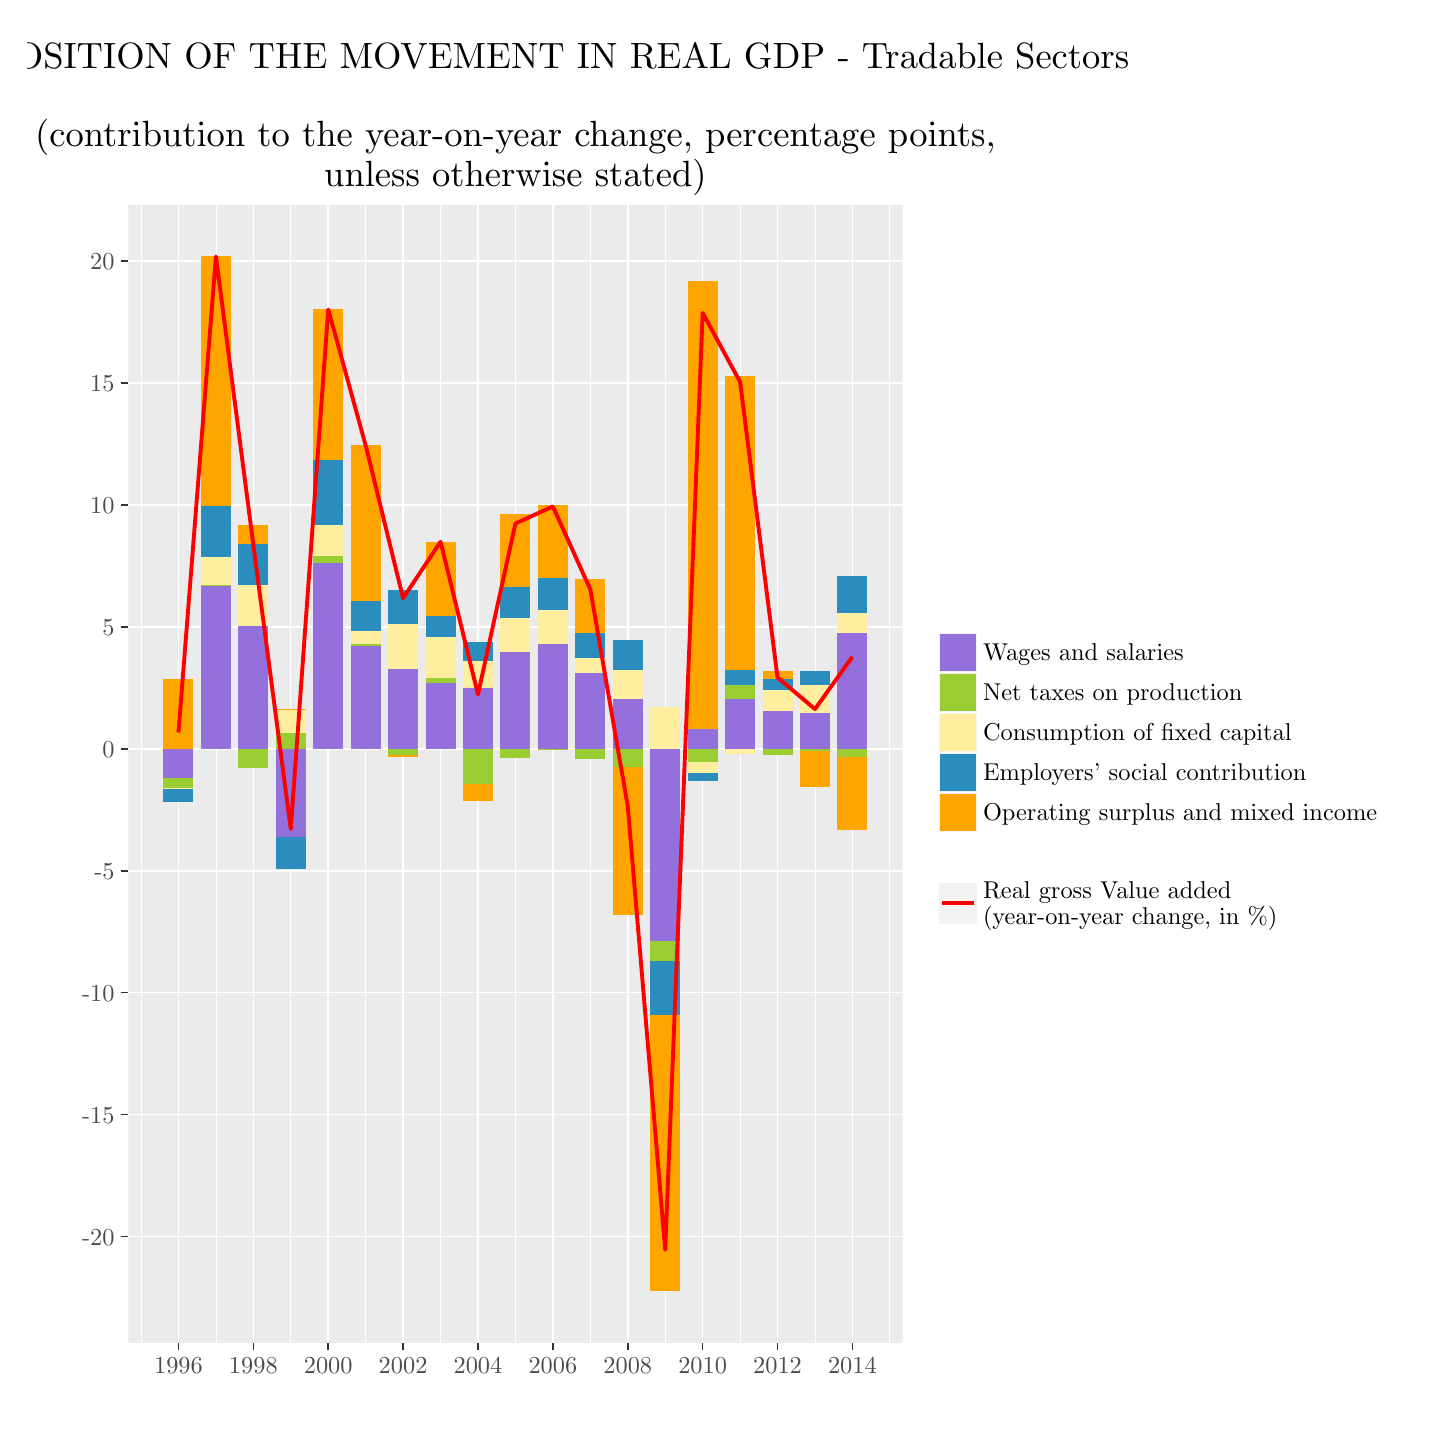
\begin{tikzpicture}[x=1pt,y=1pt]
\definecolor{fillColor}{RGB}{255,255,255}
\path[use as bounding box,fill=fillColor,fill opacity=0.00] (0,0) rectangle (505.89,505.89);
\begin{scope}
\path[clip] (  0.00,  0.00) rectangle (505.89,505.89);
\definecolor{drawColor}{RGB}{255,255,255}
\definecolor{fillColor}{RGB}{255,255,255}

\path[draw=drawColor,line width= 0.6pt,line join=round,line cap=round,fill=fillColor] (  0.00,  0.00) rectangle (505.89,505.89);
\end{scope}
\begin{scope}
\path[clip] ( 36.36, 30.69) rectangle (316.14,441.93);
\definecolor{fillColor}{gray}{0.92}

\path[fill=fillColor] ( 36.36, 30.69) rectangle (316.14,441.93);
\definecolor{drawColor}{RGB}{255,255,255}

\path[draw=drawColor,line width= 0.3pt,line join=round] ( 40.96, 30.69) --
	( 40.96,441.93);

\path[draw=drawColor,line width= 0.3pt,line join=round] ( 68.02, 30.69) --
	( 68.02,441.93);

\path[draw=drawColor,line width= 0.3pt,line join=round] ( 95.07, 30.69) --
	( 95.07,441.93);

\path[draw=drawColor,line width= 0.3pt,line join=round] (122.13, 30.69) --
	(122.13,441.93);

\path[draw=drawColor,line width= 0.3pt,line join=round] (149.19, 30.69) --
	(149.19,441.93);

\path[draw=drawColor,line width= 0.3pt,line join=round] (176.25, 30.69) --
	(176.25,441.93);

\path[draw=drawColor,line width= 0.3pt,line join=round] (203.31, 30.69) --
	(203.31,441.93);

\path[draw=drawColor,line width= 0.3pt,line join=round] (230.37, 30.69) --
	(230.37,441.93);

\path[draw=drawColor,line width= 0.3pt,line join=round] (257.43, 30.69) --
	(257.43,441.93);

\path[draw=drawColor,line width= 0.3pt,line join=round] (284.48, 30.69) --
	(284.48,441.93);

\path[draw=drawColor,line width= 0.3pt,line join=round] (311.54, 30.69) --
	(311.54,441.93);

\path[draw=drawColor,line width= 0.6pt,line join=round] ( 36.36, 69.03) --
	(316.14, 69.03);

\path[draw=drawColor,line width= 0.6pt,line join=round] ( 36.36,113.11) --
	(316.14,113.11);

\path[draw=drawColor,line width= 0.6pt,line join=round] ( 36.36,157.19) --
	(316.14,157.19);

\path[draw=drawColor,line width= 0.6pt,line join=round] ( 36.36,201.26) --
	(316.14,201.26);

\path[draw=drawColor,line width= 0.6pt,line join=round] ( 36.36,245.34) --
	(316.14,245.34);

\path[draw=drawColor,line width= 0.6pt,line join=round] ( 36.36,289.42) --
	(316.14,289.42);

\path[draw=drawColor,line width= 0.6pt,line join=round] ( 36.36,333.49) --
	(316.14,333.49);

\path[draw=drawColor,line width= 0.6pt,line join=round] ( 36.36,377.57) --
	(316.14,377.57);

\path[draw=drawColor,line width= 0.6pt,line join=round] ( 36.36,421.64) --
	(316.14,421.64);

\path[draw=drawColor,line width= 0.6pt,line join=round] ( 54.49, 30.69) --
	( 54.49,441.93);

\path[draw=drawColor,line width= 0.6pt,line join=round] ( 81.54, 30.69) --
	( 81.54,441.93);

\path[draw=drawColor,line width= 0.6pt,line join=round] (108.60, 30.69) --
	(108.60,441.93);

\path[draw=drawColor,line width= 0.6pt,line join=round] (135.66, 30.69) --
	(135.66,441.93);

\path[draw=drawColor,line width= 0.6pt,line join=round] (162.72, 30.69) --
	(162.72,441.93);

\path[draw=drawColor,line width= 0.6pt,line join=round] (189.78, 30.69) --
	(189.78,441.93);

\path[draw=drawColor,line width= 0.6pt,line join=round] (216.84, 30.69) --
	(216.84,441.93);

\path[draw=drawColor,line width= 0.6pt,line join=round] (243.90, 30.69) --
	(243.90,441.93);

\path[draw=drawColor,line width= 0.6pt,line join=round] (270.95, 30.69) --
	(270.95,441.93);

\path[draw=drawColor,line width= 0.6pt,line join=round] (298.01, 30.69) --
	(298.01,441.93);
\definecolor{fillColor}{RGB}{255,165,0}

\path[fill=fillColor] ( 49.07,245.34) rectangle ( 59.90,270.59);
\definecolor{fillColor}{RGB}{147,112,219}

\path[fill=fillColor] ( 62.60,245.34) rectangle ( 73.43,304.05);
\definecolor{fillColor}{RGB}{154,205,50}

\path[fill=fillColor] ( 62.60,304.05) rectangle ( 73.43,304.38);
\definecolor{fillColor}{RGB}{255,237,160}

\path[fill=fillColor] ( 62.60,304.38) rectangle ( 73.43,314.58);
\definecolor{fillColor}{RGB}{43,140,190}

\path[fill=fillColor] ( 62.60,314.58) rectangle ( 73.43,333.04);
\definecolor{fillColor}{RGB}{255,165,0}

\path[fill=fillColor] ( 62.60,333.04) rectangle ( 73.43,423.24);
\definecolor{fillColor}{RGB}{147,112,219}

\path[fill=fillColor] ( 76.13,245.34) rectangle ( 86.96,289.66);
\definecolor{fillColor}{RGB}{255,237,160}

\path[fill=fillColor] ( 76.13,289.66) rectangle ( 86.96,304.60);
\definecolor{fillColor}{RGB}{43,140,190}

\path[fill=fillColor] ( 76.13,304.60) rectangle ( 86.96,319.17);
\definecolor{fillColor}{RGB}{255,165,0}

\path[fill=fillColor] ( 76.13,319.17) rectangle ( 86.96,326.12);
\definecolor{fillColor}{RGB}{154,205,50}

\path[fill=fillColor] ( 89.66,245.34) rectangle (100.49,250.86);
\definecolor{fillColor}{RGB}{255,237,160}

\path[fill=fillColor] ( 89.66,250.86) rectangle (100.49,259.20);
\definecolor{fillColor}{RGB}{255,165,0}

\path[fill=fillColor] ( 89.66,259.20) rectangle (100.49,259.73);
\definecolor{fillColor}{RGB}{147,112,219}

\path[fill=fillColor] (103.19,245.34) rectangle (114.01,312.45);
\definecolor{fillColor}{RGB}{154,205,50}

\path[fill=fillColor] (103.19,312.45) rectangle (114.01,314.82);
\definecolor{fillColor}{RGB}{255,237,160}

\path[fill=fillColor] (103.19,314.82) rectangle (114.01,326.10);
\definecolor{fillColor}{RGB}{43,140,190}

\path[fill=fillColor] (103.19,326.10) rectangle (114.01,349.60);
\definecolor{fillColor}{RGB}{255,165,0}

\path[fill=fillColor] (103.19,349.60) rectangle (114.01,404.06);
\definecolor{fillColor}{RGB}{147,112,219}

\path[fill=fillColor] (116.72,245.34) rectangle (127.54,282.54);
\definecolor{fillColor}{RGB}{154,205,50}

\path[fill=fillColor] (116.72,282.54) rectangle (127.54,283.20);
\definecolor{fillColor}{RGB}{255,237,160}

\path[fill=fillColor] (116.72,283.20) rectangle (127.54,288.05);
\definecolor{fillColor}{RGB}{43,140,190}

\path[fill=fillColor] (116.72,288.05) rectangle (127.54,298.86);
\definecolor{fillColor}{RGB}{255,165,0}

\path[fill=fillColor] (116.72,298.86) rectangle (127.54,354.92);
\definecolor{fillColor}{RGB}{147,112,219}

\path[fill=fillColor] (130.25,245.34) rectangle (141.07,274.13);
\definecolor{fillColor}{RGB}{255,237,160}

\path[fill=fillColor] (130.25,274.13) rectangle (141.07,290.55);
\definecolor{fillColor}{RGB}{43,140,190}

\path[fill=fillColor] (130.25,290.55) rectangle (141.07,302.72);
\definecolor{fillColor}{RGB}{147,112,219}

\path[fill=fillColor] (143.78,245.34) rectangle (154.60,269.18);
\definecolor{fillColor}{RGB}{154,205,50}

\path[fill=fillColor] (143.78,269.18) rectangle (154.60,270.74);
\definecolor{fillColor}{RGB}{255,237,160}

\path[fill=fillColor] (143.78,270.74) rectangle (154.60,285.82);
\definecolor{fillColor}{RGB}{43,140,190}

\path[fill=fillColor] (143.78,285.82) rectangle (154.60,293.28);
\definecolor{fillColor}{RGB}{255,165,0}

\path[fill=fillColor] (143.78,293.28) rectangle (154.60,320.13);
\definecolor{fillColor}{RGB}{147,112,219}

\path[fill=fillColor] (157.31,245.34) rectangle (168.13,267.37);
\definecolor{fillColor}{RGB}{255,237,160}

\path[fill=fillColor] (157.31,267.37) rectangle (168.13,276.97);
\definecolor{fillColor}{RGB}{43,140,190}

\path[fill=fillColor] (157.31,276.97) rectangle (168.13,283.92);
\definecolor{fillColor}{RGB}{147,112,219}

\path[fill=fillColor] (170.84,245.34) rectangle (181.66,280.37);
\definecolor{fillColor}{RGB}{255,237,160}

\path[fill=fillColor] (170.84,280.37) rectangle (181.66,292.53);
\definecolor{fillColor}{RGB}{43,140,190}

\path[fill=fillColor] (170.84,292.53) rectangle (181.66,303.86);
\definecolor{fillColor}{RGB}{255,165,0}

\path[fill=fillColor] (170.84,303.86) rectangle (181.66,330.21);
\definecolor{fillColor}{RGB}{147,112,219}

\path[fill=fillColor] (184.37,245.34) rectangle (195.19,283.34);
\definecolor{fillColor}{RGB}{255,237,160}

\path[fill=fillColor] (184.37,283.34) rectangle (195.19,295.53);
\definecolor{fillColor}{RGB}{43,140,190}

\path[fill=fillColor] (184.37,295.53) rectangle (195.19,306.89);
\definecolor{fillColor}{RGB}{255,165,0}

\path[fill=fillColor] (184.37,306.89) rectangle (195.19,333.42);
\definecolor{fillColor}{RGB}{147,112,219}

\path[fill=fillColor] (197.90,245.34) rectangle (208.72,272.53);
\definecolor{fillColor}{RGB}{255,237,160}

\path[fill=fillColor] (197.90,272.53) rectangle (208.72,278.03);
\definecolor{fillColor}{RGB}{43,140,190}

\path[fill=fillColor] (197.90,278.03) rectangle (208.72,286.99);
\definecolor{fillColor}{RGB}{255,165,0}

\path[fill=fillColor] (197.90,286.99) rectangle (208.72,306.59);
\definecolor{fillColor}{RGB}{147,112,219}

\path[fill=fillColor] (211.43,245.34) rectangle (222.25,263.35);
\definecolor{fillColor}{RGB}{255,237,160}

\path[fill=fillColor] (211.43,263.35) rectangle (222.25,273.94);
\definecolor{fillColor}{RGB}{43,140,190}

\path[fill=fillColor] (211.43,273.94) rectangle (222.25,284.46);
\definecolor{fillColor}{RGB}{255,237,160}

\path[fill=fillColor] (224.95,245.34) rectangle (235.78,260.24);
\definecolor{fillColor}{RGB}{147,112,219}

\path[fill=fillColor] (238.48,245.34) rectangle (249.31,252.51);
\definecolor{fillColor}{RGB}{255,165,0}

\path[fill=fillColor] (238.48,252.51) rectangle (249.31,414.36);
\definecolor{fillColor}{RGB}{147,112,219}

\path[fill=fillColor] (252.01,245.34) rectangle (262.84,263.19);
\definecolor{fillColor}{RGB}{154,205,50}

\path[fill=fillColor] (252.01,263.19) rectangle (262.84,268.39);
\definecolor{fillColor}{RGB}{43,140,190}

\path[fill=fillColor] (252.01,268.39) rectangle (262.84,273.72);
\definecolor{fillColor}{RGB}{255,165,0}

\path[fill=fillColor] (252.01,273.72) rectangle (262.84,379.89);
\definecolor{fillColor}{RGB}{147,112,219}

\path[fill=fillColor] (265.54,245.34) rectangle (276.37,259.13);
\definecolor{fillColor}{RGB}{255,237,160}

\path[fill=fillColor] (265.54,259.13) rectangle (276.37,266.69);
\definecolor{fillColor}{RGB}{43,140,190}

\path[fill=fillColor] (265.54,266.69) rectangle (276.37,270.56);
\definecolor{fillColor}{RGB}{255,165,0}

\path[fill=fillColor] (265.54,270.56) rectangle (276.37,273.50);
\definecolor{fillColor}{RGB}{147,112,219}

\path[fill=fillColor] (279.07,245.34) rectangle (289.90,258.32);
\definecolor{fillColor}{RGB}{255,237,160}

\path[fill=fillColor] (279.07,258.32) rectangle (289.90,268.49);
\definecolor{fillColor}{RGB}{43,140,190}

\path[fill=fillColor] (279.07,268.49) rectangle (289.90,273.52);
\definecolor{fillColor}{RGB}{147,112,219}

\path[fill=fillColor] (292.60,245.34) rectangle (303.42,287.06);
\definecolor{fillColor}{RGB}{255,237,160}

\path[fill=fillColor] (292.60,287.06) rectangle (303.42,294.28);
\definecolor{fillColor}{RGB}{43,140,190}

\path[fill=fillColor] (292.60,294.28) rectangle (303.42,307.77);
\definecolor{fillColor}{RGB}{147,112,219}

\path[fill=fillColor] ( 49.07,245.34) rectangle ( 59.90,234.73);
\definecolor{fillColor}{RGB}{154,205,50}

\path[fill=fillColor] ( 49.07,234.73) rectangle ( 59.90,231.32);
\definecolor{fillColor}{RGB}{255,237,160}

\path[fill=fillColor] ( 49.07,231.32) rectangle ( 59.90,230.90);
\definecolor{fillColor}{RGB}{43,140,190}

\path[fill=fillColor] ( 49.07,230.90) rectangle ( 59.90,225.93);
\definecolor{fillColor}{RGB}{154,205,50}

\path[fill=fillColor] ( 76.13,238.23) rectangle ( 86.96,245.34);
\definecolor{fillColor}{RGB}{147,112,219}

\path[fill=fillColor] ( 89.66,245.34) rectangle (100.49,213.58);
\definecolor{fillColor}{RGB}{43,140,190}

\path[fill=fillColor] ( 89.66,213.58) rectangle (100.49,201.93);
\definecolor{fillColor}{RGB}{154,205,50}

\path[fill=fillColor] (130.25,245.34) rectangle (141.07,243.03);
\definecolor{fillColor}{RGB}{255,165,0}

\path[fill=fillColor] (130.25,243.03) rectangle (141.07,242.32);
\definecolor{fillColor}{RGB}{154,205,50}

\path[fill=fillColor] (157.31,245.34) rectangle (168.13,232.73);
\definecolor{fillColor}{RGB}{255,165,0}

\path[fill=fillColor] (157.31,232.73) rectangle (168.13,226.40);
\definecolor{fillColor}{RGB}{154,205,50}

\path[fill=fillColor] (170.84,241.84) rectangle (181.66,245.34);

\path[fill=fillColor] (184.37,244.78) rectangle (195.19,245.34);

\path[fill=fillColor] (197.90,241.66) rectangle (208.72,245.34);

\path[fill=fillColor] (211.43,245.34) rectangle (222.25,238.79);
\definecolor{fillColor}{RGB}{255,165,0}

\path[fill=fillColor] (211.43,238.79) rectangle (222.25,185.41);
\definecolor{fillColor}{RGB}{147,112,219}

\path[fill=fillColor] (224.95,245.34) rectangle (235.78,176.00);
\definecolor{fillColor}{RGB}{154,205,50}

\path[fill=fillColor] (224.95,176.00) rectangle (235.78,168.55);
\definecolor{fillColor}{RGB}{43,140,190}

\path[fill=fillColor] (224.95,168.55) rectangle (235.78,148.95);
\definecolor{fillColor}{RGB}{255,165,0}

\path[fill=fillColor] (224.95,148.95) rectangle (235.78, 49.38);
\definecolor{fillColor}{RGB}{154,205,50}

\path[fill=fillColor] (238.48,245.34) rectangle (249.31,240.39);
\definecolor{fillColor}{RGB}{255,237,160}

\path[fill=fillColor] (238.48,240.39) rectangle (249.31,236.53);
\definecolor{fillColor}{RGB}{43,140,190}

\path[fill=fillColor] (238.48,236.53) rectangle (249.31,233.79);
\definecolor{fillColor}{RGB}{255,237,160}

\path[fill=fillColor] (252.01,243.31) rectangle (262.84,245.34);
\definecolor{fillColor}{RGB}{154,205,50}

\path[fill=fillColor] (265.54,242.95) rectangle (276.37,245.34);

\path[fill=fillColor] (279.07,245.34) rectangle (289.90,244.60);
\definecolor{fillColor}{RGB}{255,165,0}

\path[fill=fillColor] (279.07,244.60) rectangle (289.90,231.46);
\definecolor{fillColor}{RGB}{154,205,50}

\path[fill=fillColor] (292.60,245.34) rectangle (303.42,242.38);
\definecolor{fillColor}{RGB}{255,165,0}

\path[fill=fillColor] (292.60,242.38) rectangle (303.42,216.12);
\definecolor{drawColor}{RGB}{255,0,0}

\path[draw=drawColor,line width= 1.4pt,line join=round] ( 54.49,251.19) --
	( 68.02,423.24) --
	( 81.54,319.01) --
	( 95.07,216.33) --
	(108.60,404.06) --
	(122.13,354.92) --
	(135.66,299.70) --
	(149.19,320.13) --
	(162.72,264.97) --
	(176.25,326.71) --
	(189.78,332.87) --
	(203.31,302.91) --
	(216.84,224.53) --
	(230.37, 64.28) --
	(243.90,402.81) --
	(257.43,377.86) --
	(270.95,271.11) --
	(284.48,259.64) --
	(298.01,278.55);
\end{scope}
\begin{scope}
\path[clip] (  0.00,  0.00) rectangle (505.89,505.89);
\definecolor{drawColor}{gray}{0.30}

\node[text=drawColor,anchor=base east,inner sep=0pt, outer sep=0pt, scale=  0.88] at ( 31.41, 66.00) {-20};

\node[text=drawColor,anchor=base east,inner sep=0pt, outer sep=0pt, scale=  0.88] at ( 31.41,110.08) {-15};

\node[text=drawColor,anchor=base east,inner sep=0pt, outer sep=0pt, scale=  0.88] at ( 31.41,154.16) {-10};

\node[text=drawColor,anchor=base east,inner sep=0pt, outer sep=0pt, scale=  0.88] at ( 31.41,198.23) {-5};

\node[text=drawColor,anchor=base east,inner sep=0pt, outer sep=0pt, scale=  0.88] at ( 31.41,242.31) {0};

\node[text=drawColor,anchor=base east,inner sep=0pt, outer sep=0pt, scale=  0.88] at ( 31.41,286.39) {5};

\node[text=drawColor,anchor=base east,inner sep=0pt, outer sep=0pt, scale=  0.88] at ( 31.41,330.46) {10};

\node[text=drawColor,anchor=base east,inner sep=0pt, outer sep=0pt, scale=  0.88] at ( 31.41,374.54) {15};

\node[text=drawColor,anchor=base east,inner sep=0pt, outer sep=0pt, scale=  0.88] at ( 31.41,418.61) {20};
\end{scope}
\begin{scope}
\path[clip] (  0.00,  0.00) rectangle (505.89,505.89);
\definecolor{drawColor}{gray}{0.20}

\path[draw=drawColor,line width= 0.6pt,line join=round] ( 33.61, 69.03) --
	( 36.36, 69.03);

\path[draw=drawColor,line width= 0.6pt,line join=round] ( 33.61,113.11) --
	( 36.36,113.11);

\path[draw=drawColor,line width= 0.6pt,line join=round] ( 33.61,157.19) --
	( 36.36,157.19);

\path[draw=drawColor,line width= 0.6pt,line join=round] ( 33.61,201.26) --
	( 36.36,201.26);

\path[draw=drawColor,line width= 0.6pt,line join=round] ( 33.61,245.34) --
	( 36.36,245.34);

\path[draw=drawColor,line width= 0.6pt,line join=round] ( 33.61,289.42) --
	( 36.36,289.42);

\path[draw=drawColor,line width= 0.6pt,line join=round] ( 33.61,333.49) --
	( 36.36,333.49);

\path[draw=drawColor,line width= 0.6pt,line join=round] ( 33.61,377.57) --
	( 36.36,377.57);

\path[draw=drawColor,line width= 0.6pt,line join=round] ( 33.61,421.64) --
	( 36.36,421.64);
\end{scope}
\begin{scope}
\path[clip] (  0.00,  0.00) rectangle (505.89,505.89);
\definecolor{drawColor}{gray}{0.20}

\path[draw=drawColor,line width= 0.6pt,line join=round] ( 54.49, 27.94) --
	( 54.49, 30.69);

\path[draw=drawColor,line width= 0.6pt,line join=round] ( 81.54, 27.94) --
	( 81.54, 30.69);

\path[draw=drawColor,line width= 0.6pt,line join=round] (108.60, 27.94) --
	(108.60, 30.69);

\path[draw=drawColor,line width= 0.6pt,line join=round] (135.66, 27.94) --
	(135.66, 30.69);

\path[draw=drawColor,line width= 0.6pt,line join=round] (162.72, 27.94) --
	(162.72, 30.69);

\path[draw=drawColor,line width= 0.6pt,line join=round] (189.78, 27.94) --
	(189.78, 30.69);

\path[draw=drawColor,line width= 0.6pt,line join=round] (216.84, 27.94) --
	(216.84, 30.69);

\path[draw=drawColor,line width= 0.6pt,line join=round] (243.90, 27.94) --
	(243.90, 30.69);

\path[draw=drawColor,line width= 0.6pt,line join=round] (270.95, 27.94) --
	(270.95, 30.69);

\path[draw=drawColor,line width= 0.6pt,line join=round] (298.01, 27.94) --
	(298.01, 30.69);
\end{scope}
\begin{scope}
\path[clip] (  0.00,  0.00) rectangle (505.89,505.89);
\definecolor{drawColor}{gray}{0.30}

\node[text=drawColor,anchor=base,inner sep=0pt, outer sep=0pt, scale=  0.88] at ( 54.49, 19.68) {1996};

\node[text=drawColor,anchor=base,inner sep=0pt, outer sep=0pt, scale=  0.88] at ( 81.54, 19.68) {1998};

\node[text=drawColor,anchor=base,inner sep=0pt, outer sep=0pt, scale=  0.88] at (108.60, 19.68) {2000};

\node[text=drawColor,anchor=base,inner sep=0pt, outer sep=0pt, scale=  0.88] at (135.66, 19.68) {2002};

\node[text=drawColor,anchor=base,inner sep=0pt, outer sep=0pt, scale=  0.88] at (162.72, 19.68) {2004};

\node[text=drawColor,anchor=base,inner sep=0pt, outer sep=0pt, scale=  0.88] at (189.78, 19.68) {2006};

\node[text=drawColor,anchor=base,inner sep=0pt, outer sep=0pt, scale=  0.88] at (216.84, 19.68) {2008};

\node[text=drawColor,anchor=base,inner sep=0pt, outer sep=0pt, scale=  0.88] at (243.90, 19.68) {2010};

\node[text=drawColor,anchor=base,inner sep=0pt, outer sep=0pt, scale=  0.88] at (270.95, 19.68) {2012};

\node[text=drawColor,anchor=base,inner sep=0pt, outer sep=0pt, scale=  0.88] at (298.01, 19.68) {2014};
\end{scope}
\begin{scope}
\path[clip] (  0.00,  0.00) rectangle (505.89,505.89);
\definecolor{fillColor}{RGB}{255,255,255}

\path[fill=fillColor] (324.68,210.80) rectangle (491.85,295.22);
\end{scope}
\begin{scope}
\path[clip] (  0.00,  0.00) rectangle (505.89,505.89);
\definecolor{drawColor}{RGB}{255,255,255}
\definecolor{fillColor}{gray}{0.95}

\path[draw=drawColor,line width= 0.6pt,line join=round,line cap=round,fill=fillColor] (328.95,272.89) rectangle (343.40,287.34);
\end{scope}
\begin{scope}
\path[clip] (  0.00,  0.00) rectangle (505.89,505.89);
\definecolor{fillColor}{RGB}{147,112,219}

\path[fill=fillColor] (329.66,273.60) rectangle (342.69,286.63);
\end{scope}
\begin{scope}
\path[clip] (  0.00,  0.00) rectangle (505.89,505.89);
\definecolor{fillColor}{RGB}{147,112,219}

\path[fill=fillColor] (329.66,273.60) rectangle (342.69,286.63);
\end{scope}
\begin{scope}
\path[clip] (  0.00,  0.00) rectangle (505.89,505.89);
\definecolor{drawColor}{RGB}{255,255,255}
\definecolor{fillColor}{gray}{0.95}

\path[draw=drawColor,line width= 0.6pt,line join=round,line cap=round,fill=fillColor] (328.95,258.43) rectangle (343.40,272.89);
\end{scope}
\begin{scope}
\path[clip] (  0.00,  0.00) rectangle (505.89,505.89);
\definecolor{fillColor}{RGB}{154,205,50}

\path[fill=fillColor] (329.66,259.14) rectangle (342.69,272.17);
\end{scope}
\begin{scope}
\path[clip] (  0.00,  0.00) rectangle (505.89,505.89);
\definecolor{fillColor}{RGB}{154,205,50}

\path[fill=fillColor] (329.66,259.14) rectangle (342.69,272.17);
\end{scope}
\begin{scope}
\path[clip] (  0.00,  0.00) rectangle (505.89,505.89);
\definecolor{drawColor}{RGB}{255,255,255}
\definecolor{fillColor}{gray}{0.95}

\path[draw=drawColor,line width= 0.6pt,line join=round,line cap=round,fill=fillColor] (328.95,243.98) rectangle (343.40,258.43);
\end{scope}
\begin{scope}
\path[clip] (  0.00,  0.00) rectangle (505.89,505.89);
\definecolor{fillColor}{RGB}{255,237,160}

\path[fill=fillColor] (329.66,244.69) rectangle (342.69,257.72);
\end{scope}
\begin{scope}
\path[clip] (  0.00,  0.00) rectangle (505.89,505.89);
\definecolor{fillColor}{RGB}{255,237,160}

\path[fill=fillColor] (329.66,244.69) rectangle (342.69,257.72);
\end{scope}
\begin{scope}
\path[clip] (  0.00,  0.00) rectangle (505.89,505.89);
\definecolor{drawColor}{RGB}{255,255,255}
\definecolor{fillColor}{gray}{0.95}

\path[draw=drawColor,line width= 0.6pt,line join=round,line cap=round,fill=fillColor] (328.95,229.52) rectangle (343.40,243.98);
\end{scope}
\begin{scope}
\path[clip] (  0.00,  0.00) rectangle (505.89,505.89);
\definecolor{fillColor}{RGB}{43,140,190}

\path[fill=fillColor] (329.66,230.23) rectangle (342.69,243.27);
\end{scope}
\begin{scope}
\path[clip] (  0.00,  0.00) rectangle (505.89,505.89);
\definecolor{fillColor}{RGB}{43,140,190}

\path[fill=fillColor] (329.66,230.23) rectangle (342.69,243.27);
\end{scope}
\begin{scope}
\path[clip] (  0.00,  0.00) rectangle (505.89,505.89);
\definecolor{drawColor}{RGB}{255,255,255}
\definecolor{fillColor}{gray}{0.95}

\path[draw=drawColor,line width= 0.6pt,line join=round,line cap=round,fill=fillColor] (328.95,215.07) rectangle (343.40,229.52);
\end{scope}
\begin{scope}
\path[clip] (  0.00,  0.00) rectangle (505.89,505.89);
\definecolor{fillColor}{RGB}{255,165,0}

\path[fill=fillColor] (329.66,215.78) rectangle (342.69,228.81);
\end{scope}
\begin{scope}
\path[clip] (  0.00,  0.00) rectangle (505.89,505.89);
\definecolor{fillColor}{RGB}{255,165,0}

\path[fill=fillColor] (329.66,215.78) rectangle (342.69,228.81);
\end{scope}
\begin{scope}
\path[clip] (  0.00,  0.00) rectangle (505.89,505.89);
\definecolor{drawColor}{RGB}{0,0,0}

\node[text=drawColor,anchor=base west,inner sep=0pt, outer sep=0pt, scale=  0.88] at (345.21,277.08) {Wages and salaries};
\end{scope}
\begin{scope}
\path[clip] (  0.00,  0.00) rectangle (505.89,505.89);
\definecolor{drawColor}{RGB}{0,0,0}

\node[text=drawColor,anchor=base west,inner sep=0pt, outer sep=0pt, scale=  0.88] at (345.21,262.63) {Net taxes on production};
\end{scope}
\begin{scope}
\path[clip] (  0.00,  0.00) rectangle (505.89,505.89);
\definecolor{drawColor}{RGB}{0,0,0}

\node[text=drawColor,anchor=base west,inner sep=0pt, outer sep=0pt, scale=  0.88] at (345.21,248.17) {Consumption of fixed capital};
\end{scope}
\begin{scope}
\path[clip] (  0.00,  0.00) rectangle (505.89,505.89);
\definecolor{drawColor}{RGB}{0,0,0}

\node[text=drawColor,anchor=base west,inner sep=0pt, outer sep=0pt, scale=  0.88] at (345.21,233.72) {Employers' social contribution};
\end{scope}
\begin{scope}
\path[clip] (  0.00,  0.00) rectangle (505.89,505.89);
\definecolor{drawColor}{RGB}{0,0,0}

\node[text=drawColor,anchor=base west,inner sep=0pt, outer sep=0pt, scale=  0.88] at (345.21,219.27) {Operating surplus and mixed income};
\end{scope}
\begin{scope}
\path[clip] (  0.00,  0.00) rectangle (505.89,505.89);
\definecolor{fillColor}{RGB}{255,255,255}

\path[fill=fillColor] (324.68,177.40) rectangle (455.83,205.11);
\end{scope}
\begin{scope}
\path[clip] (  0.00,  0.00) rectangle (505.89,505.89);
\definecolor{drawColor}{RGB}{255,255,255}
\definecolor{fillColor}{gray}{0.95}

\path[draw=drawColor,line width= 0.6pt,line join=round,line cap=round,fill=fillColor] (328.95,181.66) rectangle (343.40,197.23);
\end{scope}
\begin{scope}
\path[clip] (  0.00,  0.00) rectangle (505.89,505.89);
\definecolor{drawColor}{RGB}{255,0,0}

\path[draw=drawColor,line width= 1.4pt,line join=round] (330.39,189.45) -- (341.95,189.45);
\end{scope}
\begin{scope}
\path[clip] (  0.00,  0.00) rectangle (505.89,505.89);
\definecolor{drawColor}{RGB}{0,0,0}

\node[text=drawColor,anchor=base west,inner sep=0pt, outer sep=0pt, scale=  0.88] at (345.21,191.17) {Real gross Value added };

\node[text=drawColor,anchor=base west,inner sep=0pt, outer sep=0pt, scale=  0.88] at (345.21,181.66) {(year-on-year change, in {\%})};
\end{scope}
\begin{scope}
\path[clip] (  0.00,  0.00) rectangle (505.89,505.89);
\definecolor{drawColor}{RGB}{0,0,0}

\node[text=drawColor,anchor=base,inner sep=0pt, outer sep=0pt, scale=  1.32] at (176.25,491.30) {COMPOSITION OF THE MOVEMENT IN REAL GDP - Tradable Sectors};

\node[text=drawColor,anchor=base,inner sep=0pt, outer sep=0pt, scale=  1.32] at (176.25,477.04) {          };

\node[text=drawColor,anchor=base,inner sep=0pt, outer sep=0pt, scale=  1.32] at (176.25,462.79) {(contribution to the year-on-year change, percentage points,};

\node[text=drawColor,anchor=base,inner sep=0pt, outer sep=0pt, scale=  1.32] at (176.25,448.53) {          unless otherwise stated)};
\end{scope}
\end{tikzpicture}
